\section{Array-Based Data Structures} 

\subsection{Arrays and Lists} 

  We want to define a list that has the following methods given some list $\texttt{lst}$. 
  \begin{enumerate}
    \item $\texttt{Object y = lst.get(0)}$ outputs the $0$th element. 
    \item $\texttt{boolean y = lst.contains(elem)}$ checks if $\texttt{elem}$ 
    \item $\texttt{lst.add(Object elem)}$ adds the element to the end of the list. 
    \item $\texttt{lst.remove(Object elem)}$ removes the element. 
    \item $\texttt{lst.size()}$ returns size of the list. 
  \end{enumerate}

  \begin{definition}[ArrayList]
  An ArrayList just implements an array in the backend but with some extra systematic way to dynamically grow. If we add to an array, we either have space and can do it, or we don't and can't. If we add to an ArrayList, we can 
  \begin{enumerate}
    \item simply add to the first open position if there's space left, $O(1)$ 
    \item we grow the size of the ArrayList by creating a new larger array, copying everything, and then adding to the first open position. (linear time $O(n)$), since we have to add all the elements to the new array.
  \end{enumerate}
  Starting with a length $1$ array, if we add $N$ elements one at a time and when full, create a new array that is
  \begin{enumerate}
    \item is twice as large (geometric growth: 1, 2, 4, 8, 16, ...). Then, we must copy at sizes 1, 2, 4, 8, ... and the total values copied looks like 
    \[1 + 2 + 4 + \ldots + (N/4) + (N/2) = N - 1\]
    This is what the Java.util.ArrayList implements, and you can see the performance of adding is $O(N)$.
    \item has $1$ more position (arithmetic growth: 1, 2, 3, ...). Then, we must copy at sizes 1, 2, 3, 4, ... and the total values copied looks like
    \[1 + 2 + 3 + \ldots + (N - 1) = N (N - 1)/2\]
    If the arithmetic pattern is adding, say 1,000,000 elements, then we are wasteful of memory. 
  \end{enumerate}
  This geometric growth is a good tradeoff between performance and memory usage. It never uses more than twice the memory of an array in order to store it. Furthermore, the runtime of a geometric growth pattern is amortized constant time, which means that it is constant when averaged over a long time. This is because the vast majority of these operations are constant time, with a few add operations which require resizing to be longer. But these few ones happen less and less frequently that when averaged over a long period, we can treat it as constant. 
  \end{definition}

  One thing to note is that while adding to the end of an ArrayList can be efficient, adding to the front is not since it must shift the entire Array, even if there is space left.

  \begin{theorem}[ArrayList Runtime Complexity]
  The following are true for ArrayList $\texttt{lst}$:  
  \begin{enumerate}
      \item Getting and Contains 
      \begin{enumerate}
          \item $\texttt{lst.get(int index)}$ is $O(1)$. 
          \item Getting every element is $O(n)$ 
          \item $\texttt{lst.contains(Object elem)}$ is $O(n)$
      \end{enumerate}
      
      \item Adding 
      \begin{enumerate}
          \item $\texttt{lst.add(Object elem)}$ is amortized $O(1)$. 
          \item $\texttt{lst.add(0, Object elem)}$ is $O(n)$. 
          \item $\texttt{lst.add(int index, Object elem)}$ is on average $O(n)$. 
      \end{enumerate}
      
      \item Removing 
      \begin{enumerate}
          \item $\texttt{lst.remove(0)}$ is $O(n)$ 
          \item $\texttt{lst.remove(int index)}$ is $O(n)$ 
          \item $\texttt{lst.remove(lst.size() - 1)}$ is $O(1)$ 
          \item $\texttt{lst.remove(Object elem)}$ 
      \end{enumerate}
  \end{enumerate}
  \end{theorem}
  \begin{proof}
  Listed. 
  \begin{enumerate}
      \item Getting the element at index $\texttt{index}$ requires us to just look at the same index in the underlying array, which is $O(1)$. 
      \item We loop through each element of the ArrayList and call $\texttt{.equals(elem)}$ at each step, which results in $O(1)$. 
      \item Since the geometric growth of the ArrayList happens exponentially less frequently, it averages out to be $O(1)$, so amortized. 
      \item Adding at a specific index requires $O(n)$ since we create a new ArrayList and copy over all the elements with the added element.  
      \item Removing an object requires us to shift the indices of the remaining elements by $1$, so this is $O(n)$. 
  \end{enumerate}
  \end{proof}

  \begin{example}[String]
  The string type is just an ArrayList of characters. It has the following attributes and methods. Let $\texttt{x = "I love CS201"}$ 
  \begin{enumerate}
      \item $\texttt{int y = x.length()}$ outputs the length and is $O(1)$ 
      \item $\texttt{char y = x.charAt(0)}$ outputs a character and is $O(1)$
      \item $\texttt{String y = x.substring(0, 4)}$ 
      \item $\texttt{boolean y = x.equals("I love CS201")}$
      \item $\texttt{String y = x + "!!"}$ 
      \item $\texttt{String[] y = x.split(" ")}$
      \item $\texttt{String y = String.join(" ", words)}$
  \end{enumerate}
  \end{example}

  \begin{definition}[Linked List]
  A linked list contains a sequence of nodes that each contain an object for its element and a reference to the next node. More specifically, it can be divided up into 3 parts: 
  \begin{enumerate}
      \item The variable which points to the \textit{first} node. This can be confusing since this variable, which represents an \textit{entire list} is just a pointer to the first node. 
      \item A sequence of nodes containing the element and a reference to the next node. 
      \item The final node containing the element and a reference to $\texttt{null}$. 
  \end{enumerate}
  We can implement these functionalities in the $\texttt{ListNode}$ class, which are used to build a linked list of integers. 
  \begin{lstlisting}
  public class ListNode {
      int info;           // value i.e. element 
      ListNode next;      // reference to next ListNode
      
      ListNode(int x) {
          info = x; 
      }
      ListNode(int x, ListNode node) {
          info = x; 
          next = node; 
      }
  }
  \end{lstlisting}

  \begin{figure}[H]
    \centering 
    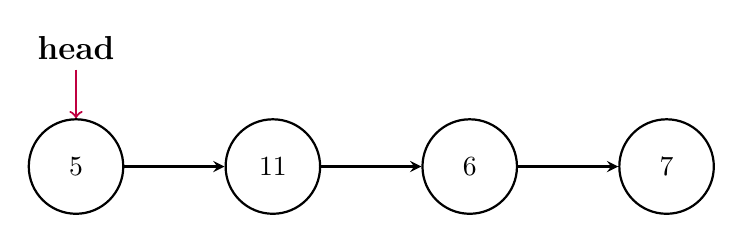
\begin{tikzpicture}[
          node/.style={circle, draw, minimum size=1.2cm, thick},
          arrow/.style={->, >=stealth, thick}
      ]

      % Nodes (circles)
      \node[node] (n1) at (0,0) {5};
      \node[node] (n2) at (2.5,0) {11};
      \node[node] (n3) at (5,0) {6};
      \node[node] (n4) at (7.5,0) {7};

      % Arrows connecting nodes
      \draw[arrow] (n1) -- (n2);
      \draw[arrow] (n2) -- (n3);
      \draw[arrow] (n3) -- (n4);

      % Head label and arrow
      \node[font=\large\bfseries] (head) at (0,1.5) {head};
      \draw[->, purple, thick] (head) -- (n1);
    \end{tikzpicture}
    \caption{The following diagram represents a linked list. } 
    \label{fig:linked_list}
  \end{figure}

  But in reality, the elements are all located random in memory and can only be found by references. 
  \end{definition}

  To print everything in a linked list, we just loop over the nodes as long as the nodes are not null. 
  \begin{lstlisting}
  public static void printList(ListNode list) {
      while (list != null) {          // common conditional for traversing 
          System.out.println(list.info); 
          list = list.next; 
      }
  }
  \end{lstlisting}

  \begin{theorem}[Linked List Runtime Complexity]
  The following are true for a basic LinkedList $\texttt{lst}$:  
  \begin{enumerate}
      \item Getting and contains 
      \begin{enumerate}
          \item $\texttt{lst.get(int index)}$ is $O(n)$ on average (unless you get the first index, which is fast).  
          \item Getting every element in the list is $O(n^2)$. 
          \item $\texttt{lst.contains(Object elem)}$ is $O(n)$ 
      \end{enumerate}
      
      \item Adding 
      \begin{enumerate}
          \item Start:  $\texttt{lst.add(0, Object elem)}$ is $O(1)$ 
          \item Middle: $\texttt{lst.add(int index, Object elem)}$ is on average $O(n)$. 
          \item End:    $\texttt{lst.add(Object elem)}$ is $O(n)$
      \end{enumerate}
      
      \item Removing 
      \begin{enumerate}
          \item Start:  $\texttt{lst.remove(0)}$ or $\texttt{lst.remove()}$ is $O(1)$ 
          \item Middle: $\texttt{lst.remove(int index)}$ is on average $O(n)$ 
          \item End:    $\texttt{lst.remove(lst.size() - 1)}$ is $O(n)$ 
      \end{enumerate}
  \end{enumerate}
  \end{theorem}
  \begin{proof}
  Listed. 
  \begin{enumerate}
      \item We must traverse from the beginning of the linked list, and so it is $O(n)$. If we just pay attention to the first (or last, for doubly-linked list) element, then this is just $O(1)$. 
      \item Getting every element is just looping an $O(n)$ operation $n$ times, so $O(n^2)$. 
      \item You need to iterate through each element and call $\texttt{.equals(elem)}$, so it is $O(n)$. 
      \item We can simply take the reference 
      \item Adding 
  \end{enumerate}
  \end{proof}

  Even though our basic LinkedList solves the problem of adding in the beginning, in order to add in the middle or end, we must get to that position (which is $O(n)$ time) before we are able to utilize our $O(1)$ add. This is quite inefficient, especially when we do repeated adding, so we should keep track of certain "markers" that indicate where our current node is. \textbf{Iterators} do this naturally, so we would like to implement some current notion of position.Below we implement a new linked list (of integers). 

  \begin{definition}[Iterator]
  An \textbf{iterator} is a Java interface that has the two methods: 
  \begin{enumerate}
      \item $\texttt{.hasnext()}$ checks if there is an element after the current one. 
      \item $\texttt{.next()}$ prints out the next element. 
  \end{enumerate}
  We want to implement iterators to any collections or whatever custom class if we want to be able to use enhanced for loops over them. 
  \end{definition}


  \begin{definition}[DIYLinkedList]
  Note the following: 
  \begin{enumerate}
      \item Adding to the end ($\texttt{add}$) and to the front ($\texttt{addtoFront}$) are both $O(1)$, since we always have access to the dynamic attributes $\texttt{first}$ and $\texttt{last}$. 
  \end{enumerate}
  \begin{lstlisting}
  public class DIYLinkedList implements Iterable<Integer> {
      private class ListNode {
          int value; 
          ListNode next; 
          public ListNode(int value) {
              this.value = value; 
          }
          public ListNode(int value, ListNode next) {
              this.value = value; 
              this.next = next; 
          }
      }
      
      private ListNode first; 
      private ListNode last; 
      private int size; 
      
      public DIYLinkedList() {
          size = 0; 
      }
      
      public int size() {
          return size; 
      }
      
      public int get(int index) {
          if (index < 0 || index >= size) {
              throw new IndexOutOfBoundsException(); 
          }
          current = first; 
          for (int i = 0; i < index; i++) {
              current = current.next; 
          }
          return current.value; 
      }
      
      public void add(int elem) { 
          // add to end 
          if (last == null) {
              last = new ListNode(elem); 
              first = last; 
          }
          else {
              last.next = new ListNode(elem); 
              last = last.next; 
          }
          size++; 
      }
      
      public void addToFront(int element) {
          // add to front 
          first = new ListNode(element, first); 
          size++; 
      }
      
      private class DIYListIterator implements Iterator<Integer> {
          ListNode current = first; 
          
          @Override 
          public boolean hasNext() {
              return current != null; 
          }
          
          @Override 
          public Integer next() {
              int value = current.value; 
              current = current.next; 
              return value; 
          }
      }
      
      @Override
      public Iterator<Integer> iterator() {
          return new DIYListIterator(); 
      }
  }
  \end{lstlisting}
  \end{definition}


  \begin{theorem}[Appending]
  Appending two ListNodes (of size $n$ and $m$) is $O(n)$ time.
  \begin{lstlisting}
  public static ListNode append(ListNode listA, ListNode listB) {
      ListNode first = listA; 
      while (listA.next != null) {
          listA = listA.next; 
      }
      listA.next = listB; 
      
      return first; 
  }
  \end{lstlisting}
  \end{theorem}

  \begin{theorem}[Reversing]
  When we reverse a linked list, we want to work with it one step at a time by establishing a \textbf{loop invariant}, which is just some condition that we want to be true every iteration. In this case, our invariant is "after $k$ iterations, $\texttt{rev}$ points to the reverse of the first $k$ nodes." 
  \begin{lstlisting}
  public ListNode reverse(ListNode front) {
      ListNode rev = null; 
      ListNode list = front; 
      while (list != null) {
          ListNode temp = list.next; 
          list.next = rev; 
          rev = list; 
          list = temp; 
      }
      return rev; 
  }
  \end{lstlisting}
  \end{theorem}

  \begin{example}
  Here are three reversing examples, in increasing difficulty: 
  \begin{enumerate}
      \item If $\texttt{front}$ is a ListNode with $\texttt{front.next == null}$, then $\texttt{reverse(front)}$ will return 
      \[\texttt{reverse(front)} \mapsto \texttt{front} \mapsto \texttt{null}\]
      \item If we have a linked list $\texttt{list} \mapsto 1 \mapsto 2 \mapsto 3 \mapsto \texttt{null}$, then $\texttt{reverse(list.next)}$ will return 
      \[\texttt{reverse(list.next)} \mapsto 3 \mapsto 2 \mapsto \texttt{null} \]
      \item If we have a linked list $\texttt{list} \mapsto 1 \mapsto 2 \mapsto 3 \mapsto \texttt{null}$, then after running $\texttt{reverse(list.next)}$, the original list variable will be 
      \[\texttt{list} \mapsto 1 \mapsto 2 \mapsto \texttt{null}\]
      This is because after the method call, we have $3 \mapsto 2 \mapsto \texttt{null}$, but the $1$ still points to $2$! Therefore, the original list, which points to $1$, will point to $2$, which points to $\texttt{null}$. 
  \end{enumerate}
  \end{example}

\subsection{Linked List}

  \begin{example}[Reverse]
    We can reverse a LinkedList with the following recursive algorithm. 
    \begin{lstlisting}
    public static ListNode reverse(ListNode list) {
        if (list == null || list.next == null) {
            return list; 
        }
        ListNode reversedLast = list.next; 
        ListNode reversedFirst = reverse(list.next); 
        reversedLast.next = list; 
        list.next = null; 
        return reversedList; 
    }
    \end{lstlisting}
  \end{example}

  \begin{example}
    The following algorithm 
    \begin{lstlisting}
    public static ListNode rec(ListNode list) {
        if (list == null || list.next == null) {
            return list; 
        }
        ListNode after = rec(list.next); 
        if (list.info <= after.info) {
            list.next = after; 
            return list; 
        }
        return after; 
    }
    \end{lstlisting}
  \end{example}

\subsection{Stacks}

  \begin{definition}[Stack]
    A \textbf{stack} is an abstract data structure represented as a \textbf{Last-In-First-Out (LIFO) list}, which implements the following methods given stack $\texttt{st}$, which we can initialize with 
    \begin{enumerate}
      \item $\texttt{st.add(Object element)}$ adds to the top of the stack, which is $O(1)$ 
      \item $\texttt{st.pop()}$ removes the element that is at the top of the stack, which is $O(1)$, and returns whatever is popped out. 
    \end{enumerate}
    Remember that this is just a list and so anything we can do with a stack we can do with a list. What makes the stack so useful is the way the list is implemented. We can literally imagine the elements of this list as "stack." If you want to remove something from the stack, of course you have to remove the top element. 
  \end{definition}

\subsection{Queues}

  \begin{definition}[Queue]
    A \textbf{queue} is an abstract data structure represented as a \textbf{First-In-First-Out (FIFO) list}, which implements the following methods given queue $\texttt{q}$, which we can initialize with Note that LinkedList implements the Queue interface. 
    \begin{enumerate}
        \item $\texttt{q.add(Object element)}$ adds to the top of the queue, referred to as \textbf{enqueue}. 
        \item $\texttt{q.remove()}$ removes the first element in the queue, referred to as \textbf{dequeue}. 
    \end{enumerate}
    This is just like how a queue works. Whatever has been waiting in the queue the longest is the one that is removed first. 
  \end{definition}

